\subsection{26 августа. Пер. Кичкинекол Малый (1А)}
\textit{Метеоусловия: утром переменная облачность, днём, вечером сильный лождь, ветер.}


\begin{figure}[h!]
	\centering
	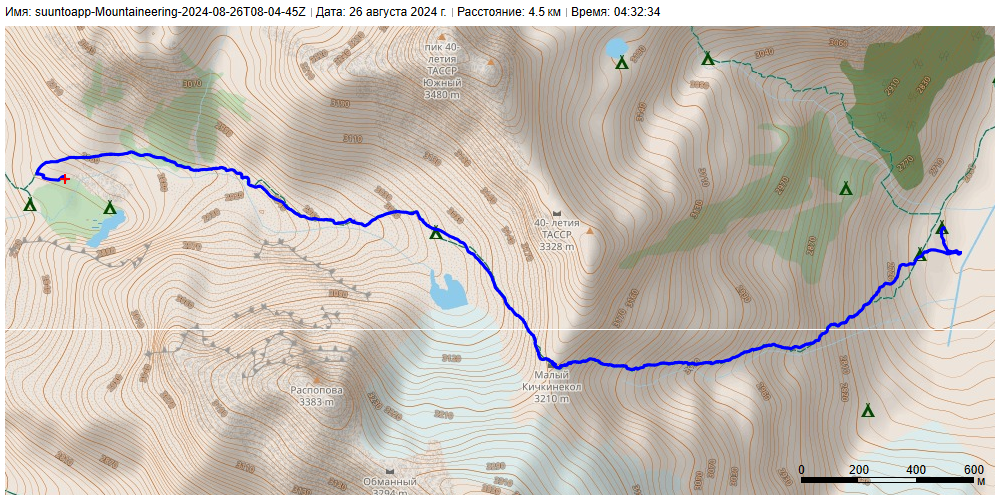
\includegraphics[angle=0, width=0.7\linewidth]{../pics/mini_maps/26}
	\label{fig:mini_26}
\end{figure}

Подъём в 08:00. Гроза закончилась, небо затянуто облаками, периодически выходит солнце. Выходим в 11:00, движемся по тропе, траверсирующей травянистый склон.

\begin{figure}[h!]
	\centering
	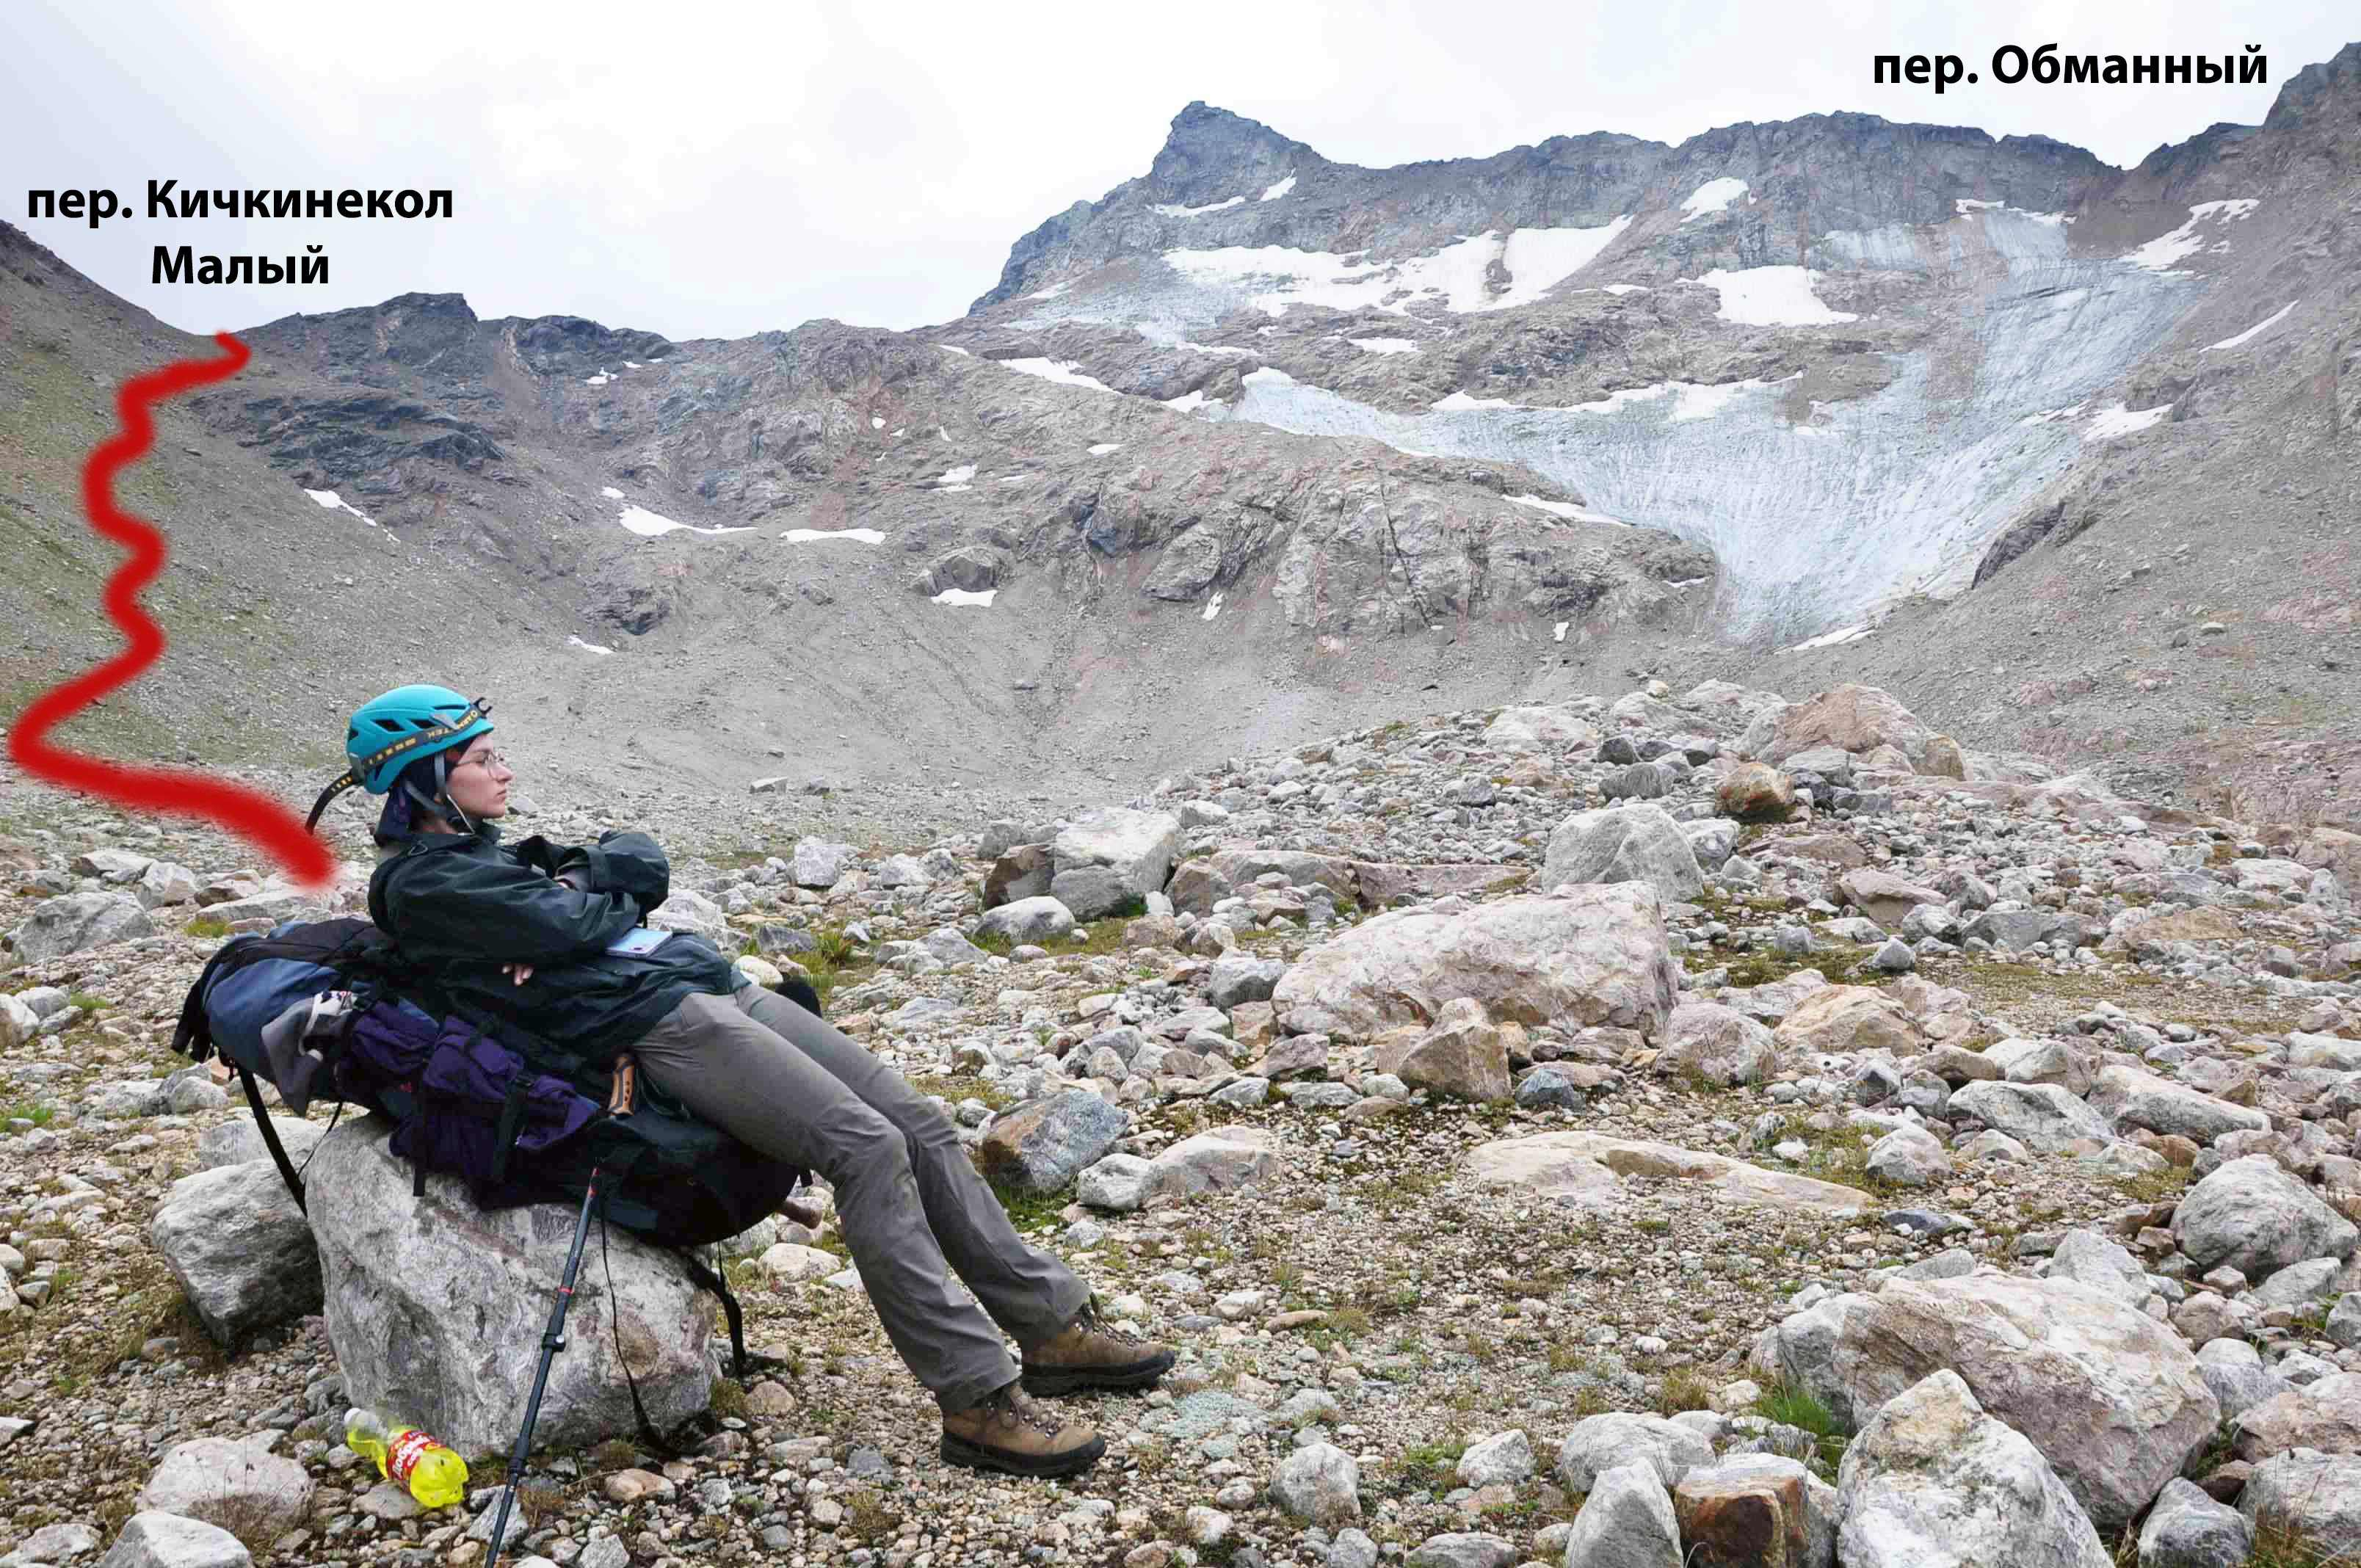
\includegraphics[width=0.7\linewidth]{../pics/DSC_0226}
	\caption{Маршрут движения группы}
	\label{fig:DSC_0226}
\end{figure}

 Тропа обходит водопад на западной оконечности поляны слева пхд. Встречаются туры, тропу видно хорошо. Постепенно травянистый склон переходит в морену, погода ухудшается, начинается небольшой дождь.

\begin{figure}[h!]
	\centering
	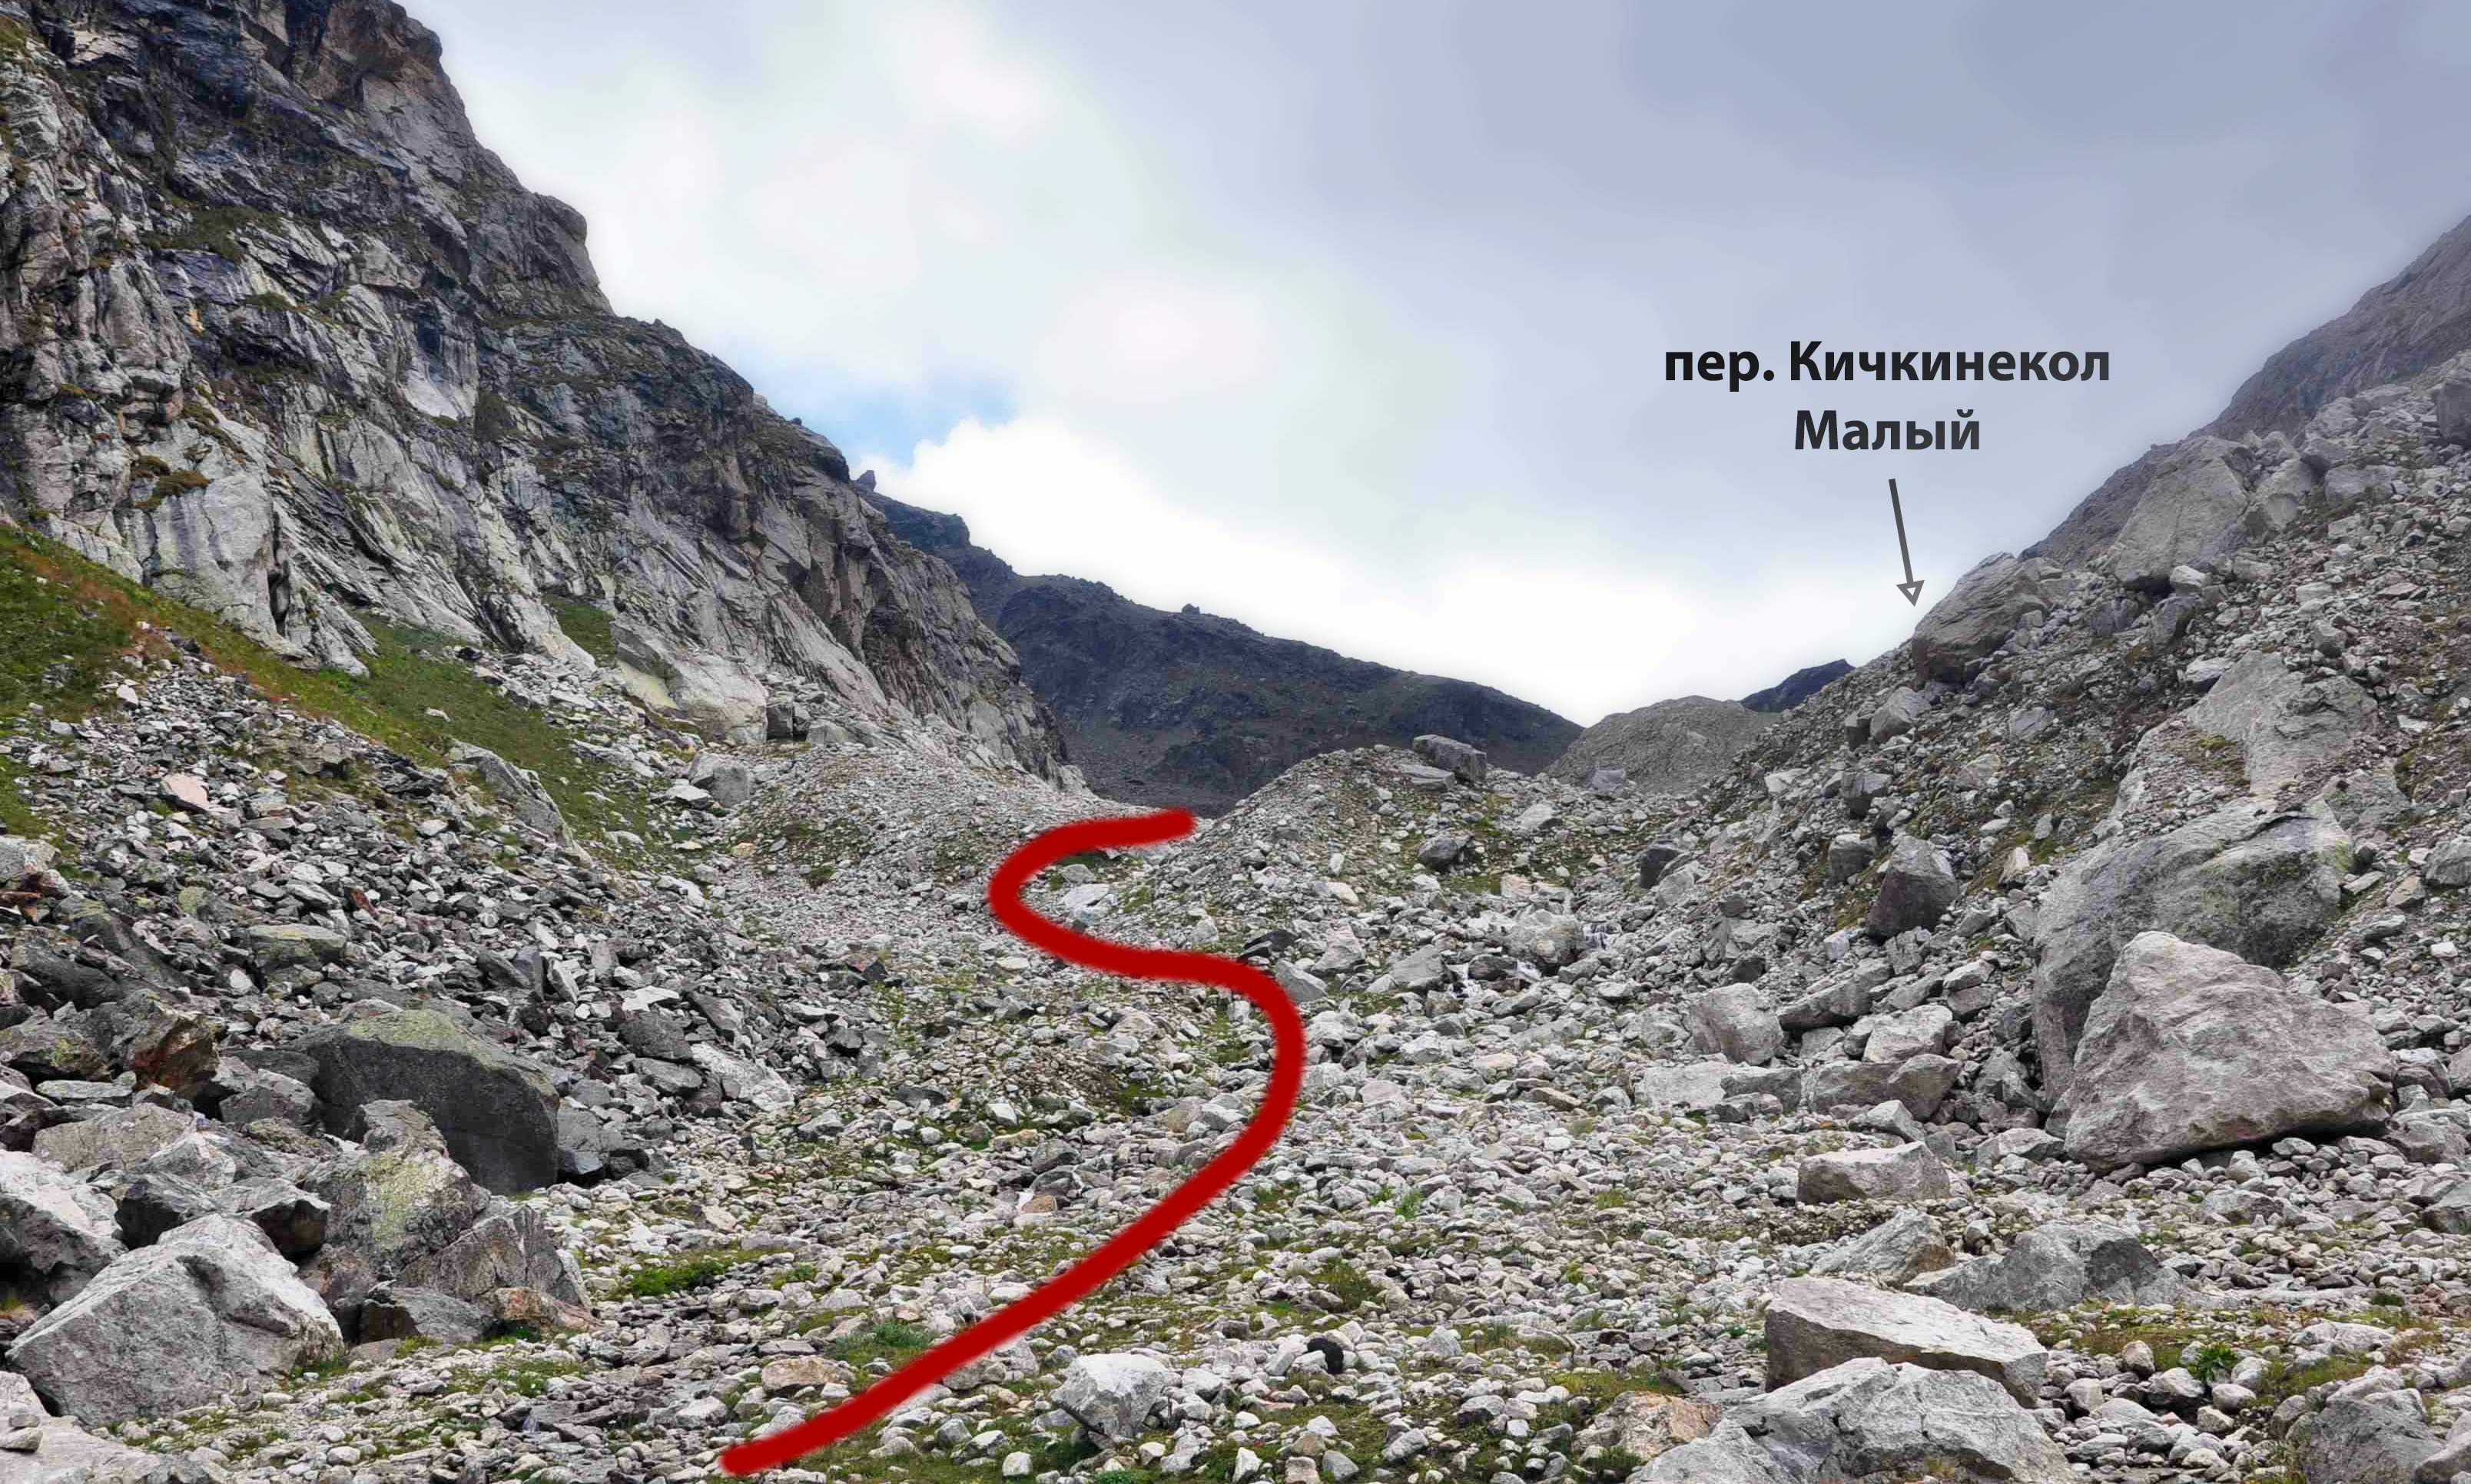
\includegraphics[width=0.7\linewidth]{../pics/DSC_0221.JPG}
	\caption{Путь подъема на перевал}
	\label{fig:DSC_0221}
\end{figure}

\begin{figure}[h!]
	\centering
	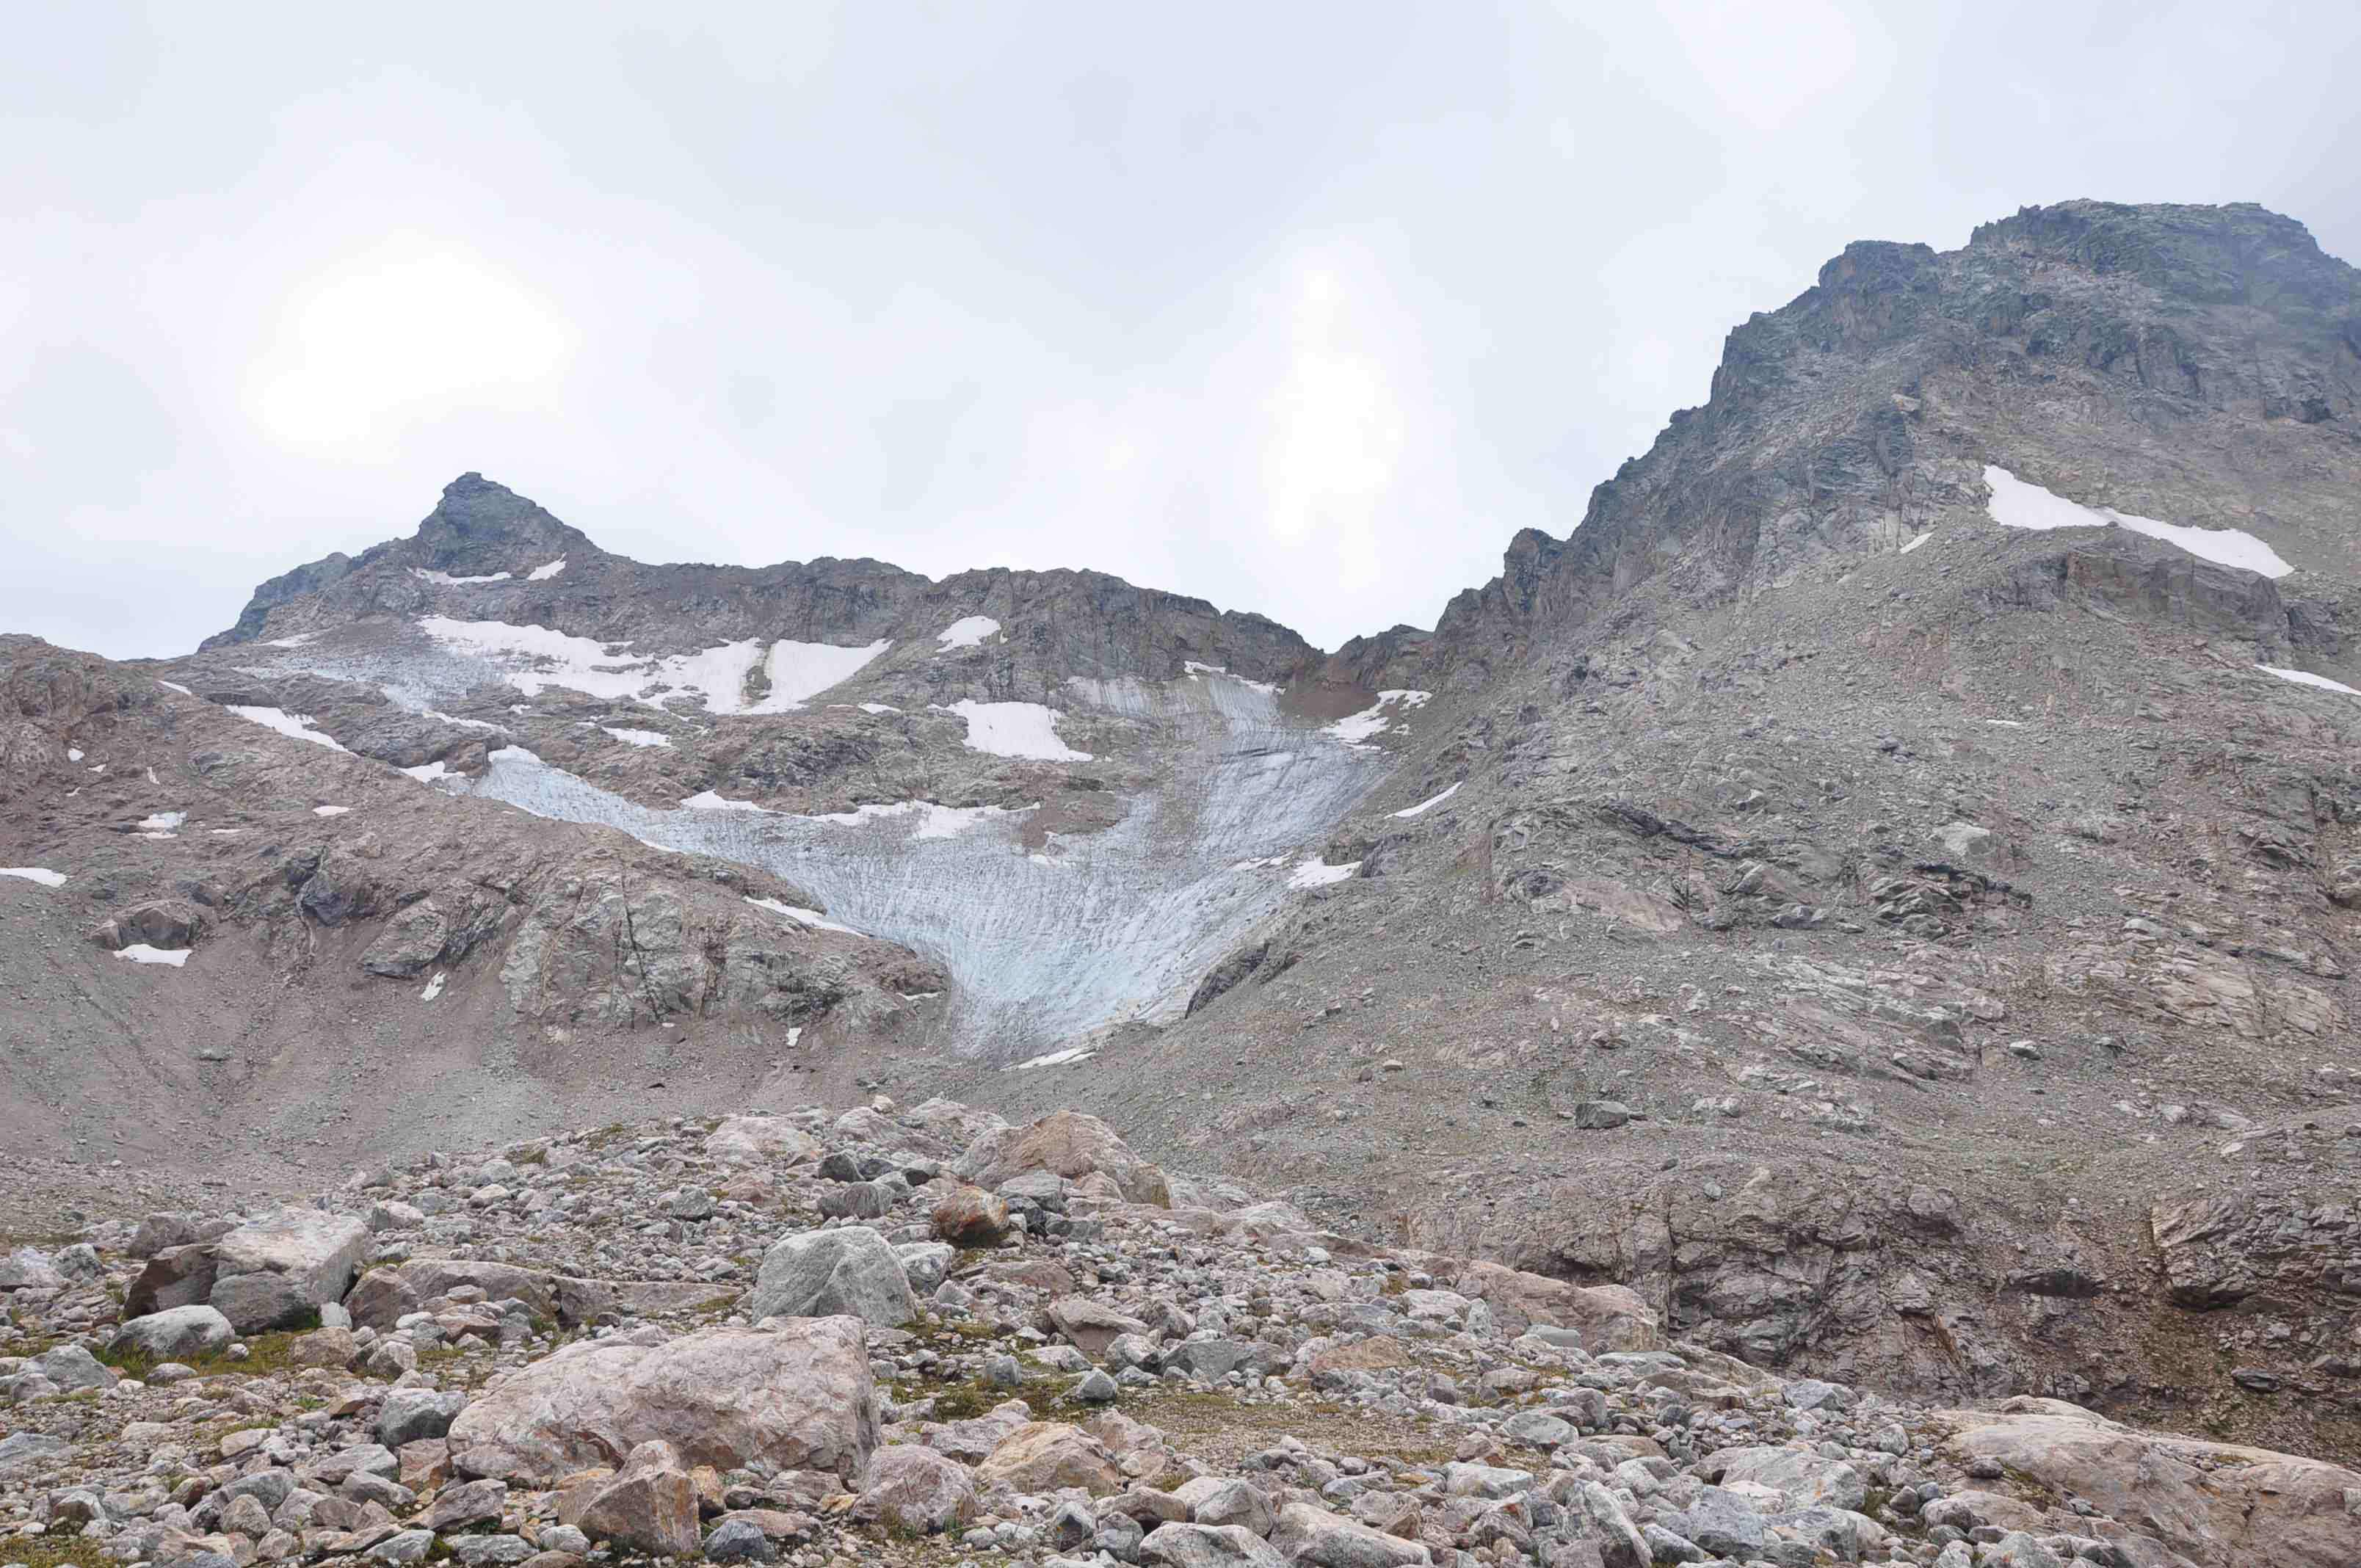
\includegraphics[width=0.7\linewidth]{../pics/DSC_0227.JPG}
	\caption{Цирк пер. Обманный справа пхд от пер. Кичкинекол Малый}
	\label{fig:DSC_0227}
\end{figure}

\begin{figure}[h!]
	\centering
	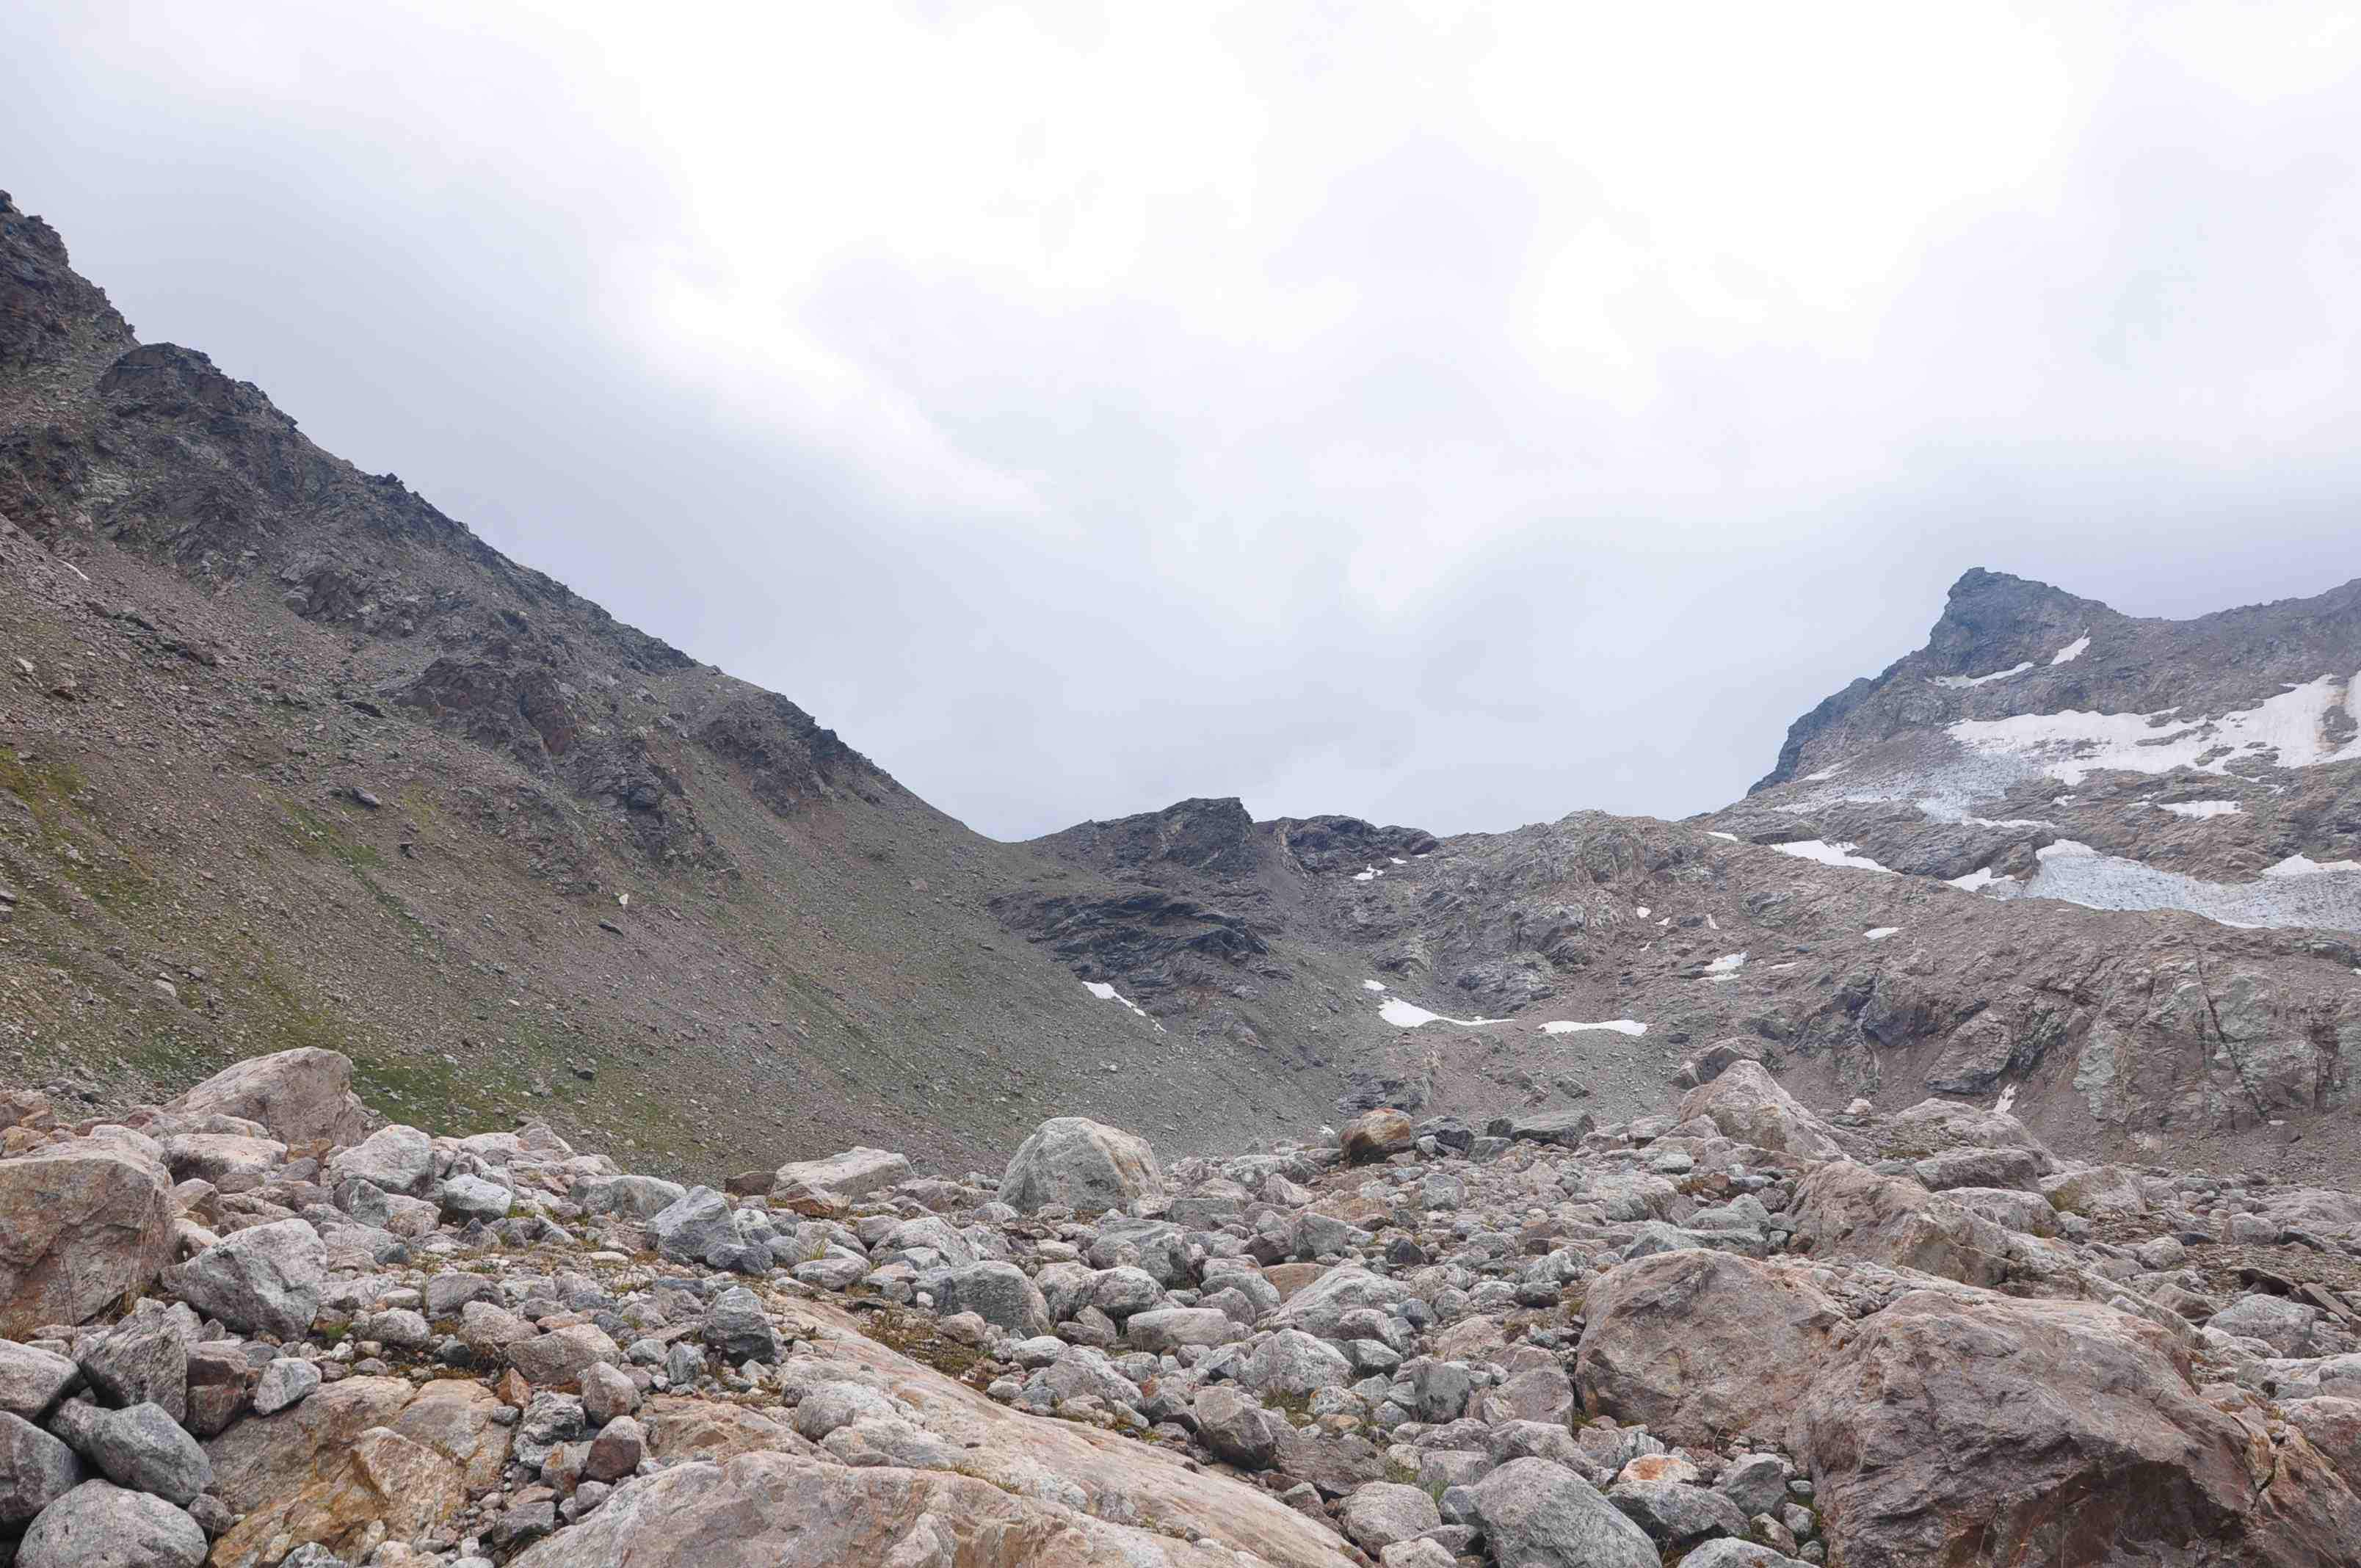
\includegraphics[width=0.7\linewidth]{../pics/DSC_0230.JPG}
	\label{fig:DSC_0230}
\end{figure}

\begin{figure}[h!]
	\centering
	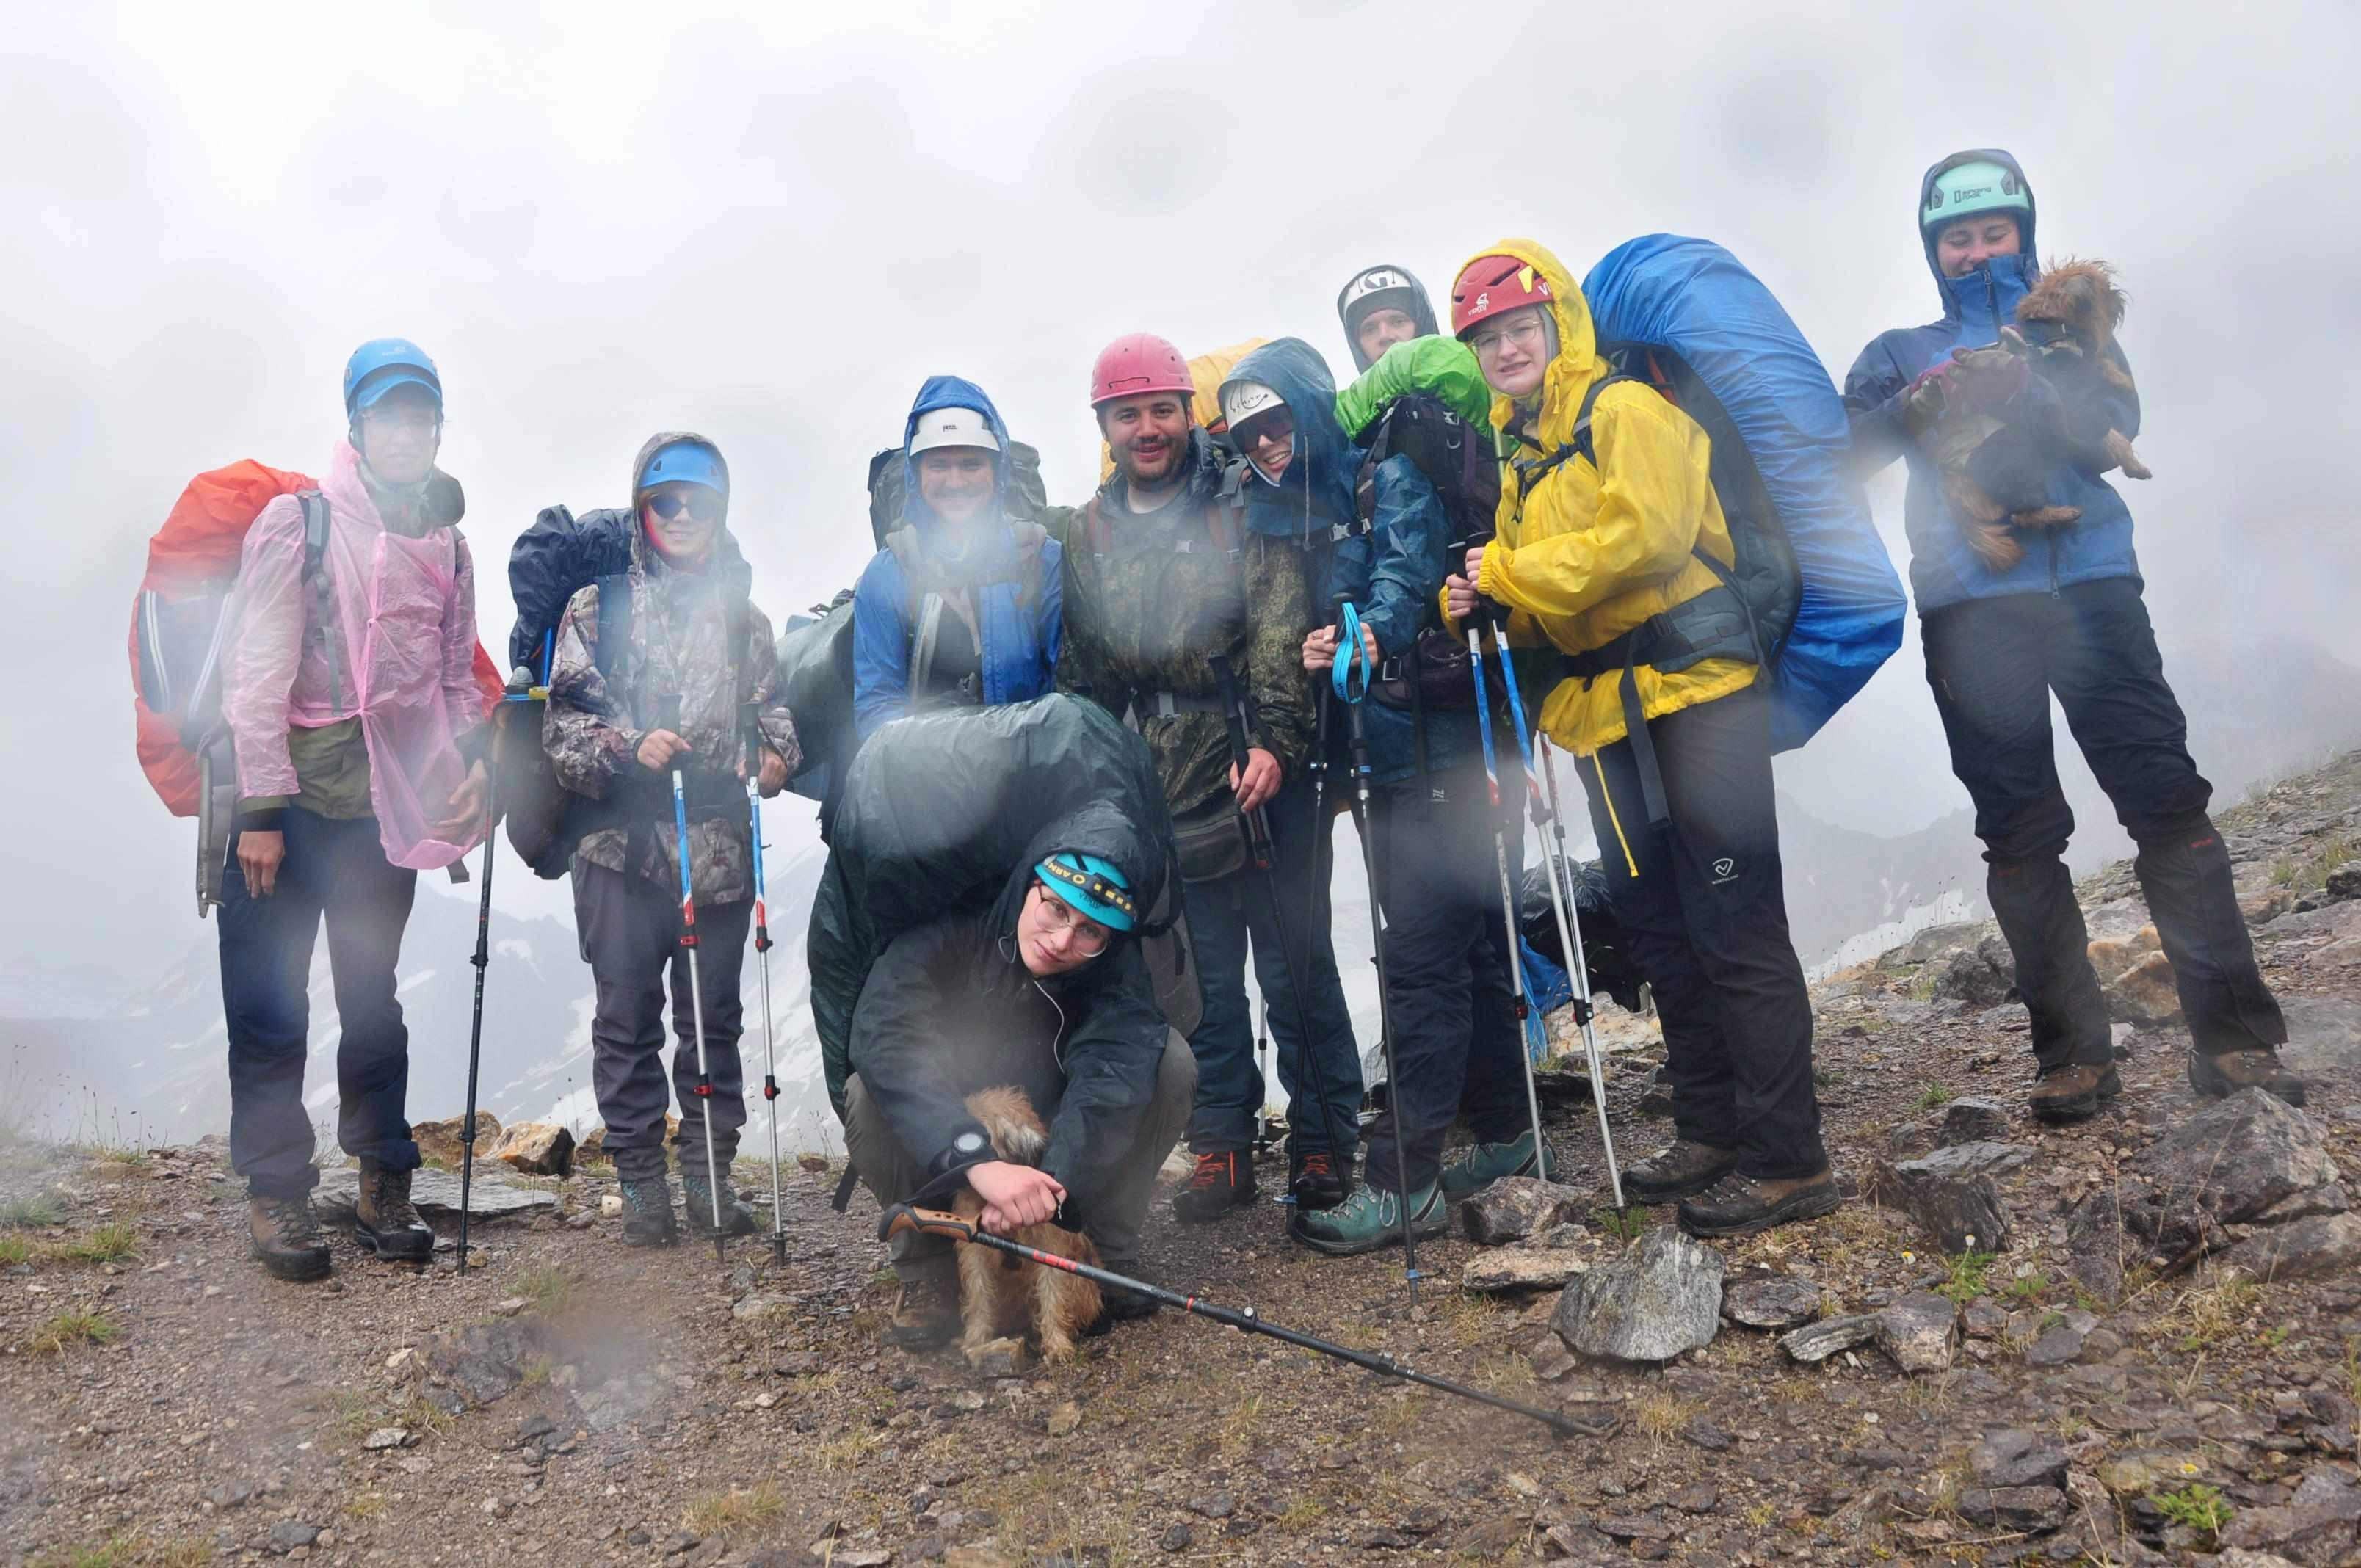
\includegraphics[angle=0, width=0.7\linewidth]{../pics/DSC_0239.JPG}
	\label{fig:DSC_0239}
\end{figure}

\begin{figure}[h!]
	\centering
	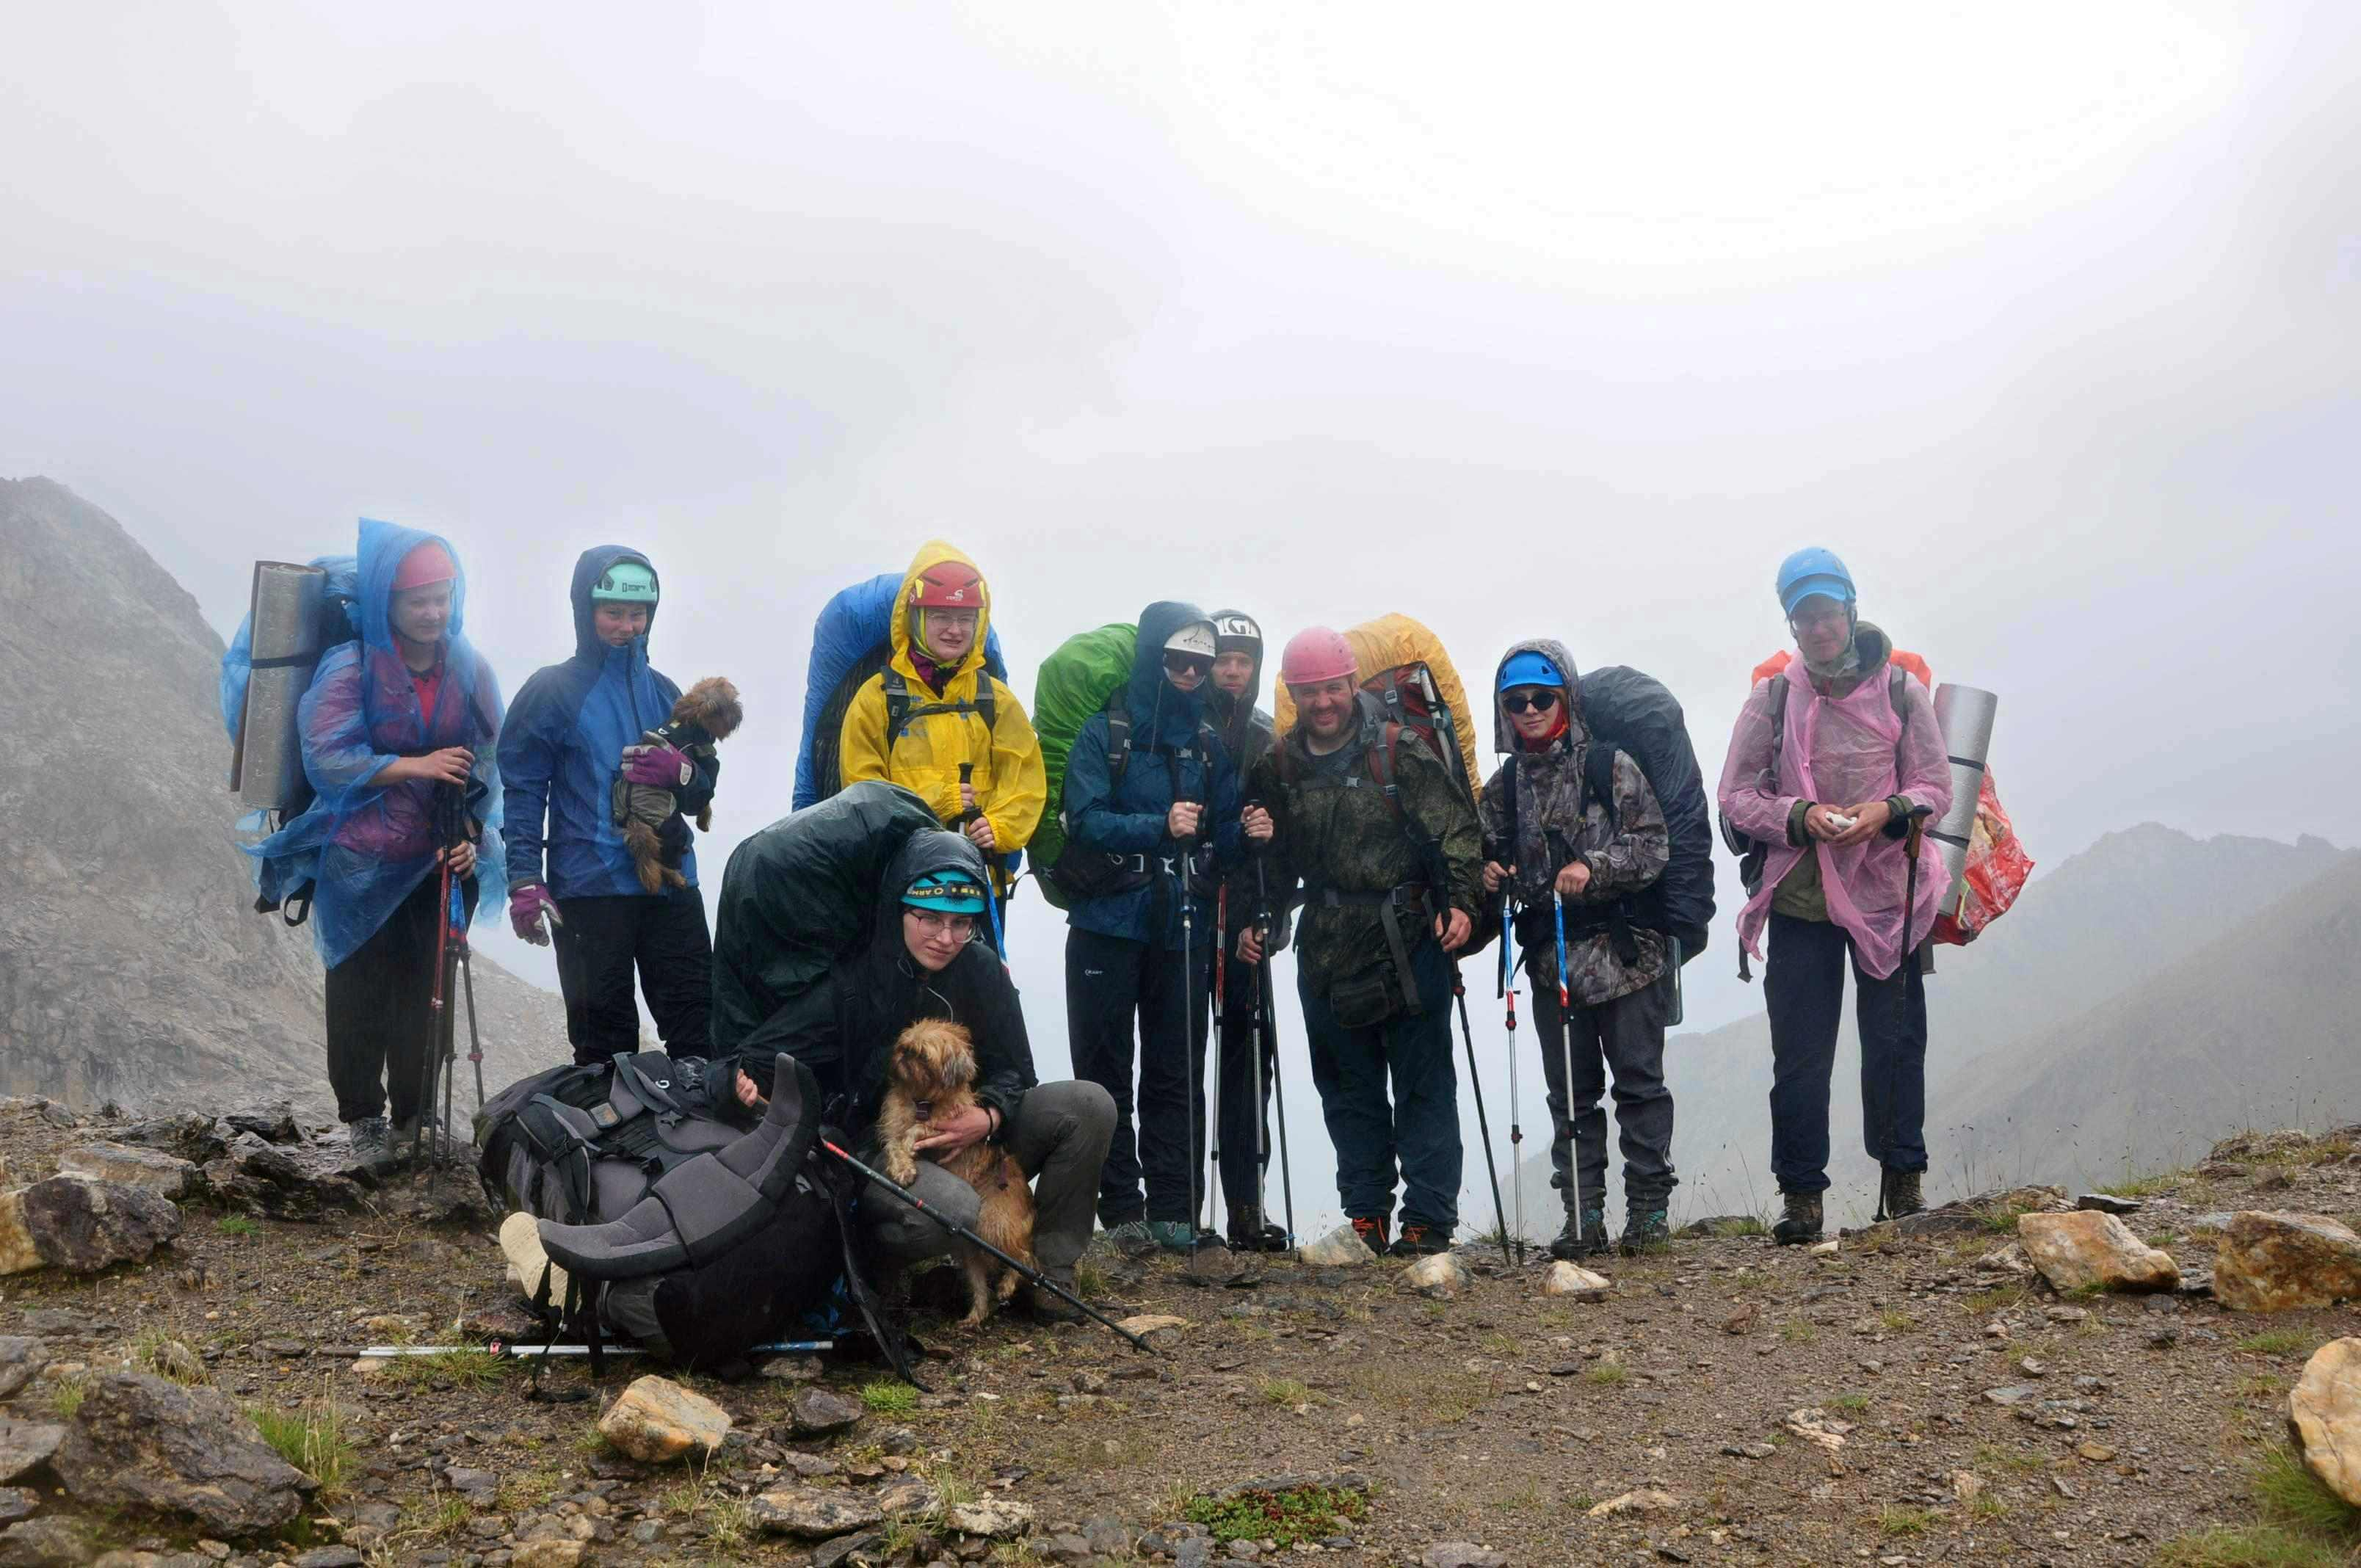
\includegraphics[angle=0, width=0.7\linewidth]{../pics/DSC_0242.JPG}
	\label{fig:DSC_0242}
\end{figure}

\clearpage